\documentclass{article}
\usepackage{color}
\usepackage{hyperref}
\usepackage{graphicx}
\usepackage{etoolbox}
\usepackage{my_package}

%define filter for product 1 
\newif\ifproductOne
\expandafter\ifstrequal\expandafter{\jobname}{p1}{\productOnetrue}{\productOnefalse}

%define filter for product 2
\newif\ifproductTwo
\expandafter\ifstrequal\expandafter{\jobname}{p2}{\productTwotrue}{\productTwofalse}

%define filter for product 3
\newif\ifproductThree
\expandafter\ifstrequal\expandafter{\jobname}{p3}{\productThreetrue}{\productThreefalse}

\begin{document}
\section{Produktvarianten}
\begin{itemize}
\item Produkt: Emaildienst
\begin{itemize}
\item Produkt 1: \productOne
\item Produkt 2: \productTwo
\item Produkt 3: \productThree
\end{itemize}
\item Anmeldung 
\begin{itemize}
\item \productOne : Anmeldung über Email
\item \productTwo : Anmeldung über Google-Konto
\item \productThree : Anmeldung über Facebook-Konto  
\end{itemize}
\item Preis 
\begin{itemize}
\item Produkt 1: 5 CHF pro Monat
\item Produkt 2: 10 CHF pro Monat
\item Produkt 3: 100 CHF pro Jahr
\end{itemize}
\item Mindestlaufzeit
\begin{itemize}
\item Produkt 1: keine Mindestlaufzeit
\item Produkt 2: 3 Monate
\item Produkt 3: 1 Jahr 
\end{itemize}
\end{itemize}
\section{Filter in einer Liste}

\begin{enumerate}
	\item Gehen Sie zu \textbf{\textcolor{blue}{www.\manufacturer.com}}
	\item In der oberen linken Ecke wählen Sie die Schaltfläche 
\includegraphics[height=\baselineskip]{log_in}.
	\begin{itemize}
		\item Das Dialogfeld \textbf{\textcolor{blue}{Anmeldung}} erscheint. Siehe Abbildung \ref{fig:log_in}
	\end{itemize}	 
	%Schritt für Produkt 1	
	\ifproductOne
	\item In dem Feld \textbf{\textcolor{blue}{Email}}, geben Sie Ihre Email Adresse ein. 
	\else
	\fi
%Schritt für Produkt 2
	\ifproductTwo
	\item In dem Feld \textbf{\textcolor{blue}{Google user}}, geben Sie Ihren Google-Benutzernamen 		ein. 
	\else
	\fi
%Schritt für Produkt 3
	\ifproductThree
	\item In dem Feld \textbf{\textcolor{blue}{Facebook user}}, geben Sie Ihren Facebook-Benutzernamen ein. 
	\else
	\fi
	\item In dem Feld \textbf{\textcolor{blue}{Passwort}}, begen Sie Ihr Passwort ein. 
	\item Beenden Sie mit der Schaltfläche \textbf{\textcolor{blue}{Anmelden}}
\end{enumerate}
\section{Filter in einer Tabelle}
\begin{table}[h]
\begin{center}
\begin{tabular}{l l }
\textbf{Feature} & \textbf{Beschreibung} \\
\hline \hline
Volumen & 10 GB\\
\ifproductOne
Preis & 5 CHF pro Monat \\
\else
\fi
\ifproductTwo
Preis & 10 CHF pro Monat \\
\else
\fi
\ifproductThree
Preis & 100 CHF pro Jahr \\
\else
\fi
Support & 24h\\
\ifproductOne
Anmeldung & Email\\
\else
\fi
\ifproductTwo
Anmeldung & Google-User\\
\else
\fi
\ifproductThree
Anmeldung & Facebook-User\\
\else
\fi
\end{tabular}
\end{center}
\end{table}

\section{Filter auf eine Abbildung}
\begin{figure}
\begin{center}


\ifproductOne
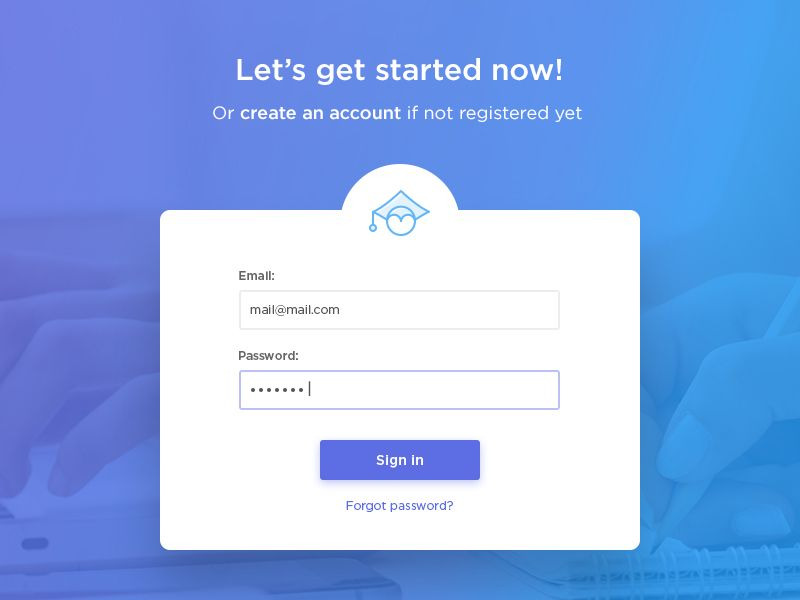
\includegraphics[scale=0.5]{log_in_email}
\else

\fi
\ifproductTwo
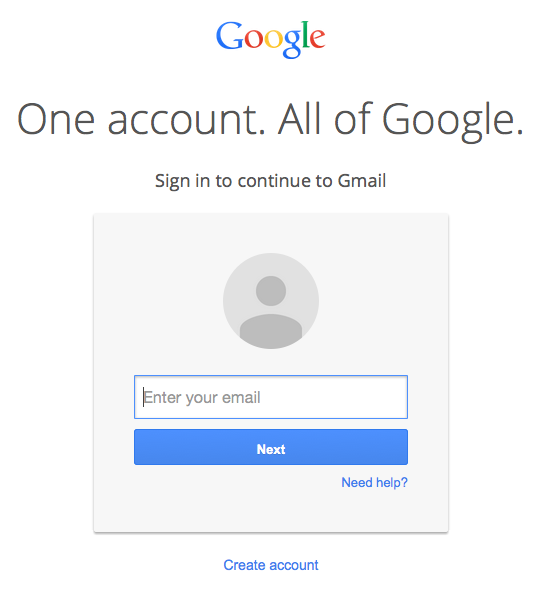
\includegraphics[scale=0.5]{log_in_google}
\else

\fi
\ifproductThree
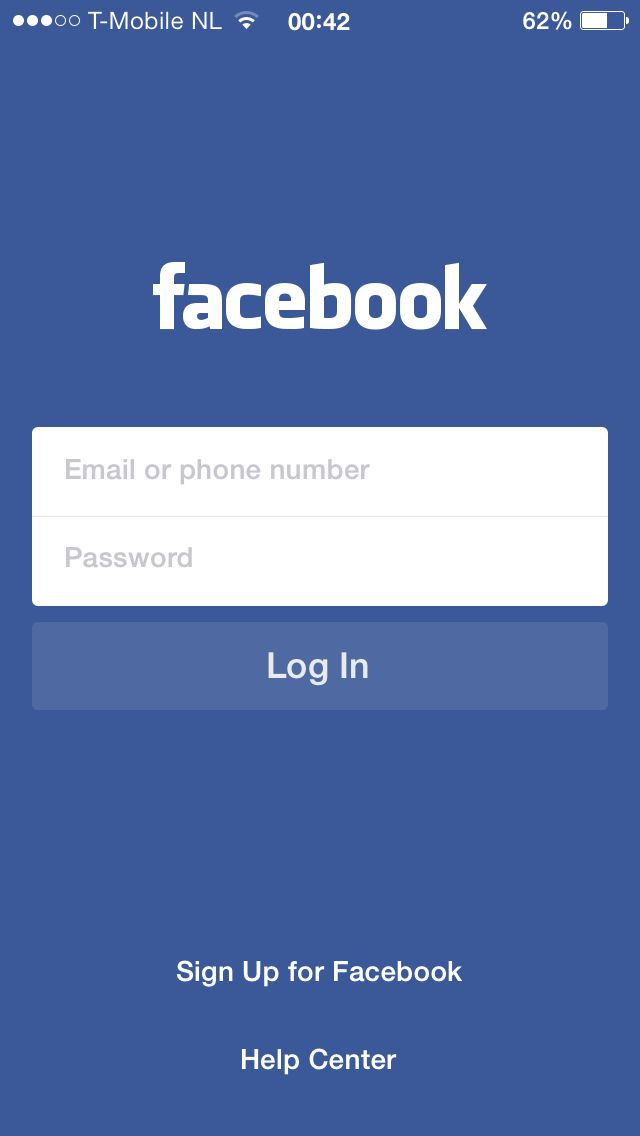
\includegraphics[scale=0.5]{log_in_facebook}
\else

\fi
\caption{Dialog Anmeldung}
\end{center}
\label{fig:log_in}
\end{figure}
\section{Filter auf Paragraph}
\end{document}